%! Licence = CC BY-NC-SA 4.0

%! Author = gianfluetsch
%! Date = 30. Dez 2021
%! Project = cydef_summary


\section{Forensic Readiness}
Unter Forensic Readiness versteht man die technische und organisatorische Vorbereitung, um im Fall eines Sicherheitsvorfalls schnell und zielgerichtet reagieren und eine IT-forensische Nachuntersuchung optimal durchführen zu können.

\subsection{Forensic Readiness Analyse}
Es sollte eine genaue IST-Analyse der IT-Landschaft durchgeführt, alle bestehenden Richtlinien überprüft und die relevanten Prozesse für den Umgang mit IT-Sicherheitsverletzungen erstellt/ überprüft werden. So kann ermittelt werden, ob die bestehenden organisatorischen und technischen Strukturen eine adäquate Reaktion auf sicherheitsrelevante Ereignisse zulassen.\\

\begin{itemize}
    \item Welche potentiellen Angriffsszenarien sind relevant (Threat Model)?
    \item Welche Daten müssen im Notfall verfügbar sein?
    \item Wie sehen die optimalen organisatorischen Voraussetzungen dafür aus?
    \item Wie sehen die optimalen technischen Voraussetzungen dafür aus?
\end{itemize}

\subsubsection{Forensic Readiness Optimierung}
Auf Basis der Analyse können wirkungsvolle Maßnahmen, um sowohl die organisatorischen als auch die technischen Voraussetzungen zu optimieren, erarbeitet werden. Dazu gehört die Umsetzung der Maßnahmen, das erstellen von Checklisten und z.B. auch die entsprechende Schulung der Mitarbeiter.\\

\begin{itemize}
    \item Integration von forensischen Datensicherungen in den Incident Response Prozesse
    \item IT-Richtlinien, die für die Forensic Readiness von Relevanz sind
    \item Umsetzung der Massnahmen
    \item Erstellen von Checklisten
    \item Notwendige Vereinbarungen mit IT-Dienstleistern
    \item Schulung der Mitarbeiter
\end{itemize}

\subsection{Web Forensic Readiness}

\subsubsection{Topologie}
Client $\rightarrow$ WAF $\rightarrow$ APP $\rightarrow$ API $\rightarrow$ DB
\begin{center}
    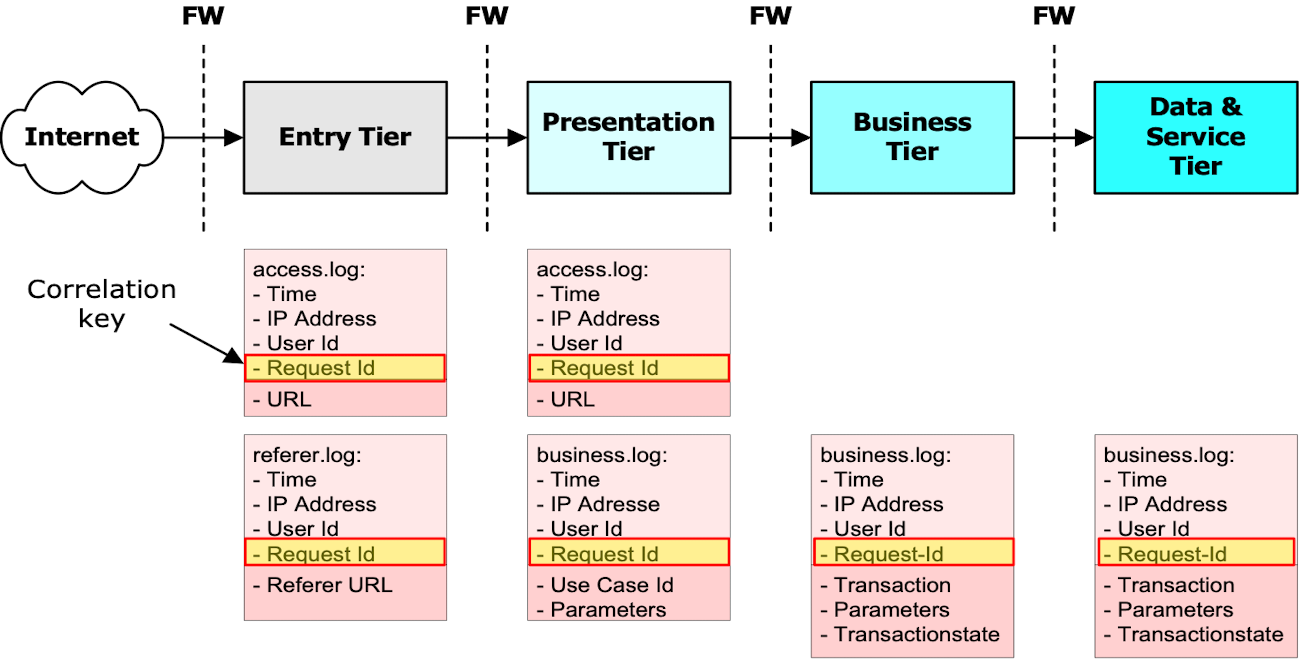
\includegraphics[width=1.0\linewidth]{./img/08-forensic_readiness/web_fr}
    \vspace{-8pt}
\end{center}

\subsubsection{Ablauf Request}
\begin{enumerate}
    \item Request zu WAF $\rightarrow$ \textit{Unique\_ID} wird generiert und an Request \glqq angehängt\grqq
    \item Request weiter an APP mit \textit{Unique\_ID} (APP muss diese ID loggen)
    \item Request weiter zu API mit \textit{Unique\_ID} (API muss diese auch loggen)
    \item Request weiter zu DB mit \textit{Unique\_ID} (DB muss diese auch loggen)\\
\end{enumerate}
\vspace{-8pt}
\textbf{Damit kann über die geloggte \textit{Unique\_ID} nachträglich der Weg jedes Requests herausgefunden und analysiert werden.}

\subsubsection{Unique-ID zum Logfile hinzufügen}
2 verschiedene Arten möglich:
\begin{itemize}
    \item Vorkonfigurierte Protokollrichtlinie ,,ForensicLog`` verwenden (nicht konfigurierbar)
    \item Hinzufügen einer UNIQUE-ID zum benutzerdefinierten Protokoll (sehr flexibel)
\end{itemize}

\subsubsection{Unique-ID Vorteile}
\begin{itemize}
    \item Korrelation von Ereignissen zwischen Multi-Tier- und Mikro-Service-Architekturen
    \item Weil ein Zeitstempel nicht ausreicht
    \item Der erste Server (der dem Internet zugewandt ist) sollte die Unique-ID generieren und sie in die eigenen Protokolldateien aufnehmen. Außerdem sollte die Unique-ID an die Backend-Dienste weitergegeben werden, in der Regel durch Hinzufügen eines speziellen Headers. Die Backend-Dienste sollten die Unique-ID parsen und zu den eigenen Protokollen hinzufügen. Außerdem sollte er die Unique-ID jedem weiteren Server oder jeder weiteren Instanz hinzufügen. Wenn dies bei allen Diensten der Fall wäre, könnten Sie jederzeit herausfinden, wer, wann, wo etwas passiert ist.
    \item Ohne die Unique-ID sind Unternehmen aufgeschmissen und müssen sich auf Zeitstempel verlassen.
\end{itemize}


\subparagraph{Forensic rediness}

\subsection{Forensic Readiness Apache Reverse Proxy}
Distributed systems, and those using microservices architectures in particular, scatter the order's log messages further, across multiple locations, to be gathered by centralised logging tools. To make it straightforward to investigate problems, you need a way to group the log messages that relate to a particular order, in all of your systems or services.

\subsubsection{Unique-ID}
Correlation IDs provide the standard solution to this problem. A correlation ID uniquely identifies each \glqq customer order\grqq, or the equivalent in your system. Similarly, web-based applications have \glqq user requests\grqq, for each user interaction

\subsubsection{How do you enable the unique-id in the apache?}
By using the \lstinline|mod_unique_id| module.

\subsubsection{How do you log the unique-id into the forensic log}
\lstinline|mod_log_forensic| is included in most distribution packages of Apache and comes with the source tarball download, but if you compile Apache 2.x.x from source, you need to add \lstinline|--enable-log-forensic| and \lstinline|--enable-unique-id| to the configure line.

\subsubsection{How do you inject the unique-id to the backend service?}
By adding the \textit{UNIQUE\_ID} into the following Request Header towards to backend service. On both parts it will be logged for logs/ time correlation.

